%!TEX root = ../../thesis.tex

\section{Eniric: Extended \nir information content}
\label{sec:eniric}
Here the software developed to compute the {RV} precisions is presented.
It is an extension of the code used for the calculations of~\citet{figueira_radial_2016}, hence ``extended'' in the name.
This section documents the vast improvements (optimizations and extensions) made to the software.
Changes made that affect the derived {RV} precision attained are specifically documented in detail, with the relative precision changes provided.
This work resulted in a submission of a publication\footnote{Available at \href{http://joss.theoj.org/papers/384bfc031df47ecef2d88328f63e5479}{http://joss.theoj.org/papers/384bfc031df47ecef2d88328f63e5479}} to \emph{The Journal of Open Source Software}\footnote{\href{http://joss.theoj.org/}{joss.theoj.org/}} (JOSS) {Neal and Figueria 2018 (in prep.)} with the source code openly available on \href{Github}{https://github.com/jason-neal/eniric}.


\subsection{Automated testing}
\label{subsec:automated_testing}
Before the changes to the software are detailed, a note about software testing.
Automated software testing is an important practise to insure that the code written is correct, and that new changes to not break the previously written code.
This practice is crucial in computer science and professional software engineering but seldom encouraged or practised in scientific programming~\cite{storer_bridging_2017}.
It is however starting to becoming increasingly encouraged as part of the movement towards open and reproducible science.

After inheriting the code-base from \citet{figueira_radial_2016}, software tests were added for a number of purposes: to learn and explore the code-base, to check and test the original functionality, and to identify if any changes implemented break the original functionality.
Version control practises were used to incrementally add small separate changes to the code base at a time, regularly testing in a continuous integration manor.
This is done by sending the code-base to a repository\footnote{public or private} on Github\footnote{\href{https://bitbucket.org}{Bitbucket} and \href{https://gitlab.com}{GitLab} are other popular options}.
Automated tools and services then forward the project to testing, code style checking, or other continuous-integration services (e.g.\ \href{https://travis-ci.com}{Travis-CI}) which either run the automated tests, or other checks on each new change.
The public Travis-CI record of the test for \eniric{} can be found at \href{https://travis-ci.org/jason-neal/eniric}{https://travis-ci.org/jason-neal/eniric}.

This process was valuable in preventing the introduction of errors, but also in identifying and errors in the~\citep{figueira_radial_2016} results which are outlined in \cref{subsec:condition_two_bug}.
Based on this experience it is a practise that is highly recommend for scientific programming.


\subsection{Performance}
\label{subsec:code_performance}
The software performance is one aspect that was addressed in the upgrades.
The original code used in~\citet{figueira_radial_2016} was very slow, taking around two hours per parameter combination.
This led to multiple weeks worth of processing time required to compute the {RV} precision for the original paper (180 combinations).
The latest implementation of \eniric{} can compute all 180 combinations in less than two hours.

The major performance bottleneck was identified in the convolution stage.
Stating with a \numpy{} array containing the spectrum the algorithm looped though each pixel in the spectrum, selecting a suitable window around the given pixel with a \emph{comprehension list}\footnote{Example usage can be found \href{https://docs.python.org/3/tutorial/datastructures.html\#list-comprehensions}{here}.}.
The output is a list\footnote{A list is a native Python data structure.} which was turned back into a \numpy{} array, eventually summed and then appended to a new list.
This list was once again converted into \numpy{} array.
The main performance issue is a Python implementation detail to do with a type checking overhead when converting between \numpy{} and native data types.
These conversions were performed 2--3 times for every pixel in the large spectral arrays of order \({10}^{4}\) pixels.

Remaining entirely in the fast compiled \numpy{} code and not changing data types a performance gain of around 250\(\times\)\,X was achieved.
This is done by using boolean masks instead of comprehension lists and pre-allocating a \numpy{} array to store the results a itself.

The convolution computation of individual pixels is an ``embarrassingly parallel''\footnote{\href{https://en.wikipedia.org/wiki/Embarrassingly\_parallel}{https://en.wikipedia.org/wiki/Embarrassingly\_parallel}} problem.
What this means is that convolution result for pixel $i+1$ does not depend on the convolution result obtained of pixel $i$, each can be computed independently.
Therefore, parallel processing was also added into the convolution to further improve the performance, roughly dividing the convolution time by the number of processors used.

As the convolution step is the main bottleneck, caching of the convolution results was included using the \href{https://joblib.readthedocs.io}{Joblib} package.
Caching the convolution function stores the input parameters and the convolution result together.
If the same input parameters are passed to the convolution function again, it fetches the computed results from memory, rather than recomputing the time intensive convolutions.
This avoids unnecessary wasted computation time computing the same convolution results, improving the performance of repeated runs of the software.

The \emph{PyAstronomy} package has a ``slow'' version of the rotational convolution, which has a wavelength dependent kernel as done here.
They also provide ``fast'' convolution kernels that used fixed kernel, taking the central wavelength value.
These are significantly faster but are only valid for very short wavelength regions, in which the kernels do not significantly change.
They are not deemed suitable for use in this work due to the large wavelength span of spectroscopic bands and the wavelength dependant spacing of the spectra considered here.
A comparison of the performance between the \emph{PyAstronomy} convolutions and the convolutions implemented in \eniric{} and used here are provided in a \emph{Jupyter} notebook in the Github repository of ``eniric''\footnote{\href{https://github.com/jason-neal/eniric/blob/master/docs/Notebooks/Convolution_speeds.ipynb}{}}, basically they fall in between the ``fast'' and ``slow'' implementation of \emph{PyAstronomy}.



\subsection{Model extension}
\label{subsec:eniric_model_extesion}
The original software hard-coded the range of models computed, specifically by identifying the spectra by their spectral types (M0--M9) and the specific \Vsini{} and resolution values.

The software was made more suitable to future computations, by allowing any spectrum in the {PHOENIX-ACES} library grid to be analysed, provided the four identifying parameters [\Teff, \Logg, \feh{}, $\aleph$ \alphafe{}]. 

Later this was also extended to include the {BT-Settl} library spectra.
\# Handle any {PHOENIX} aces models.


\section{Numerical Gradient}
\label{sec:numerical_gradient}
One of the key insights from \cref{eqn:optimal_weight,eqn:dv_rms} is that the radial velocity error is inversely proportional gradient of the spectra, In numerically computing the {RV} precision, the result is slightly dependent on the numerical method used to compute the gradient.
In the original code used in~\citet{figueira_radial_2016} the gradient or slope is approximated using the forward finite difference method.
The \numpy{} package provides a function to calculate the gradient using a more advanced methods that compute a more precise gradient.
In this section \todo{we} explore the affect of improving the precision of the numerical gradient on the final {RV} precision.

The simplest way to calculate the derivative using finite difference methods~\citep{quarteroni_numerical_2000}.
These arising from the Newton's definition of the derivative for a continuous function \(f(x)\) which should be familiar from introductory calculus:
\[f'(x) = \lim_{h \to 0} \frac{f(x+h)-f(x)}{h}~.\]

There are three common varieties of the finite difference,
\begin{equation}
{FFD} = \frac{f(x+h)-f(x)}{h}, {CFD}=\frac{f(x+\frac{1}{2}h)-f(x-\frac{1}{2}h)}{h}, {BFD}=\frac{f(x)-f(x-h)}{h}\,,
\end{equation}
called the forwards ({FFD}), central ({CFD}), and backwards ({BFD}) finite differences respectively.
The order of uncertainty on the {FFD}/{BFD} is \(\mathcal{O}(h)\) while for the {CFD} it is \(\mathcal{O}({h}^{2})\)~\citep{quarteroni_numerical_2000}.
As the wavelength spacing between samples/pixels (h) is small the {CFD} will a more precise value for the gradient at each pixel.

In this case \(h\) is the difference in wavelength between the two pixels considered.
In the {FFD} case the gradient at pixel \(i\) becomes:
\begin{equation}
\frac{\partial {A}_{0}(i)}{\partial\lambda(i)} = \frac{{A}_{0}(i+1) - {A}_{0}(i)}{\lambda(i+1)-\lambda(i)}, \hspace{2em} 1 \leq i \leq n-1.
\label{eqn:ffd_precision}
\end{equation}
At each pixel the numerical derivative is evaluated to be the average slope between itself and the following pixel and is an approximation to the derivative.
This only extends to \(i= n-1\), where \(n\) is the number of points in the spectrum, and the last pixel is dropped from the {RV} calculation.\footnote{This is important in the case of Condition~\#2.}


The \emph{gradient}\footnote{Documentation available at \href{https://docs.scipy.org/doc/numpy/reference/generated/numpy.gradient.html\#id1 }{https://docs.scipy.org/doc/numpy/reference/generated/numpy.gradient.html\#id1}}  method provided in \numpy{} contains a more advanced numerical methods to calculate the derivative.
It uses a \textit{compact difference} method~\citep{quarteroni_numerical_2000} which expand the finite differences using a Taylor expansion and then selecting coefficients to minimize the \textit{consistency error}.
From the \numpy{} documentation the consistency error here is \[\eta_i = \partial{f(x_i)}/\partial{x} -  [\alpha f(x_i) + \beta f(x_i +h_d) + \gamma f(x_i - h_s)],\] where \(h_s\) and \(h_d\) are the spacing to the left and right of \(i\) respectively.
With Taylor expansion this turns into solving a linear system of equations:
\[\begin{cases}
\alpha + \beta + \gamma = 0\\
-\beta {h_d} + \gamma {h_s} = 1\\
\beta {h_{d}}^{2} + \gamma {h_{s}}^{2} = 0
\end{cases}
\]
which result in the approximation of the gradient of the central values to be

\[\frac{\partial{f(x_i)}}{\partial{x}} = \frac{{h_{s}}^{2}f\left(x_{i} + {h_{d}}\right) + \left({h_{d}}^{2} - {h_{s}}^{2}\right)f\left(x_{i}\right) - {h_{d}}^{2}f\left(x_{i}-{h_{s}}\right)} {{h_{s}}{h_{d}}\left({h_{d}} + {h_{s}}\right)} + \mathcal{O}\left(\frac{h_{d}{h_{s}}^{2} + {h_{s}}{h_{d}}^{2}}{{h_{d}} + {h_{s}}}\right) \label{full_compact_difference}.\]

If the spectrum is evenly spaced ${h_{s}}={h_{d}}$  reduces to the standard second order {CFD} approximation:

\[\frac{\partial{f(x_i)}}{\partial{x}} = \frac{f\left(x_{i+1}\right) - f\left(x_{i-1}\right)}{2h} + \mathcal{O}\left({h}^{2}\right)\]


Applying this to the situation presented here, similar to \cref{eqn:ffd_precision}, results in:
\[\frac{\partial {A}_{0}(i)}{\partial\lambda(i)} = \frac{{\lambda(i-1)}^{2} {A}_{0}(i+1) + ({\lambda(i+1)}^{2}-{\lambda(i-1)}^{2}) {A}_{0}(i) - {\lambda(i+1)}^{2} {A}_{0}(i-1)} {\lambda(i-1)\lambda(i+1)(\lambda(i+1) + \lambda(i-1))}, \hspace{1em} 2 \leq i \leq n-1\]

with an uncertainty of \(\mathcal{O}\left(\frac{\lambda(i+1){\lambda(i-1)}^{2} + \lambda(i-1){\lambda(i+1)}^{2}}{\lambda(i+1) + \lambda(i-1)}\right)\).


{\red{} Wavelength spacing \(\delta\lambda\) between pixels is a function of \(\lambda\), Resolution and sampling choices.
    Can I do something with this??}

The \emph{gradient} function from \numpy{} implements central differences for the interior points, accurate to second order, and first order accurate one-sided (forward or backward) differences at the boundaries, computed using the same compact difference procedure.

\begin{figure}
    \centering
    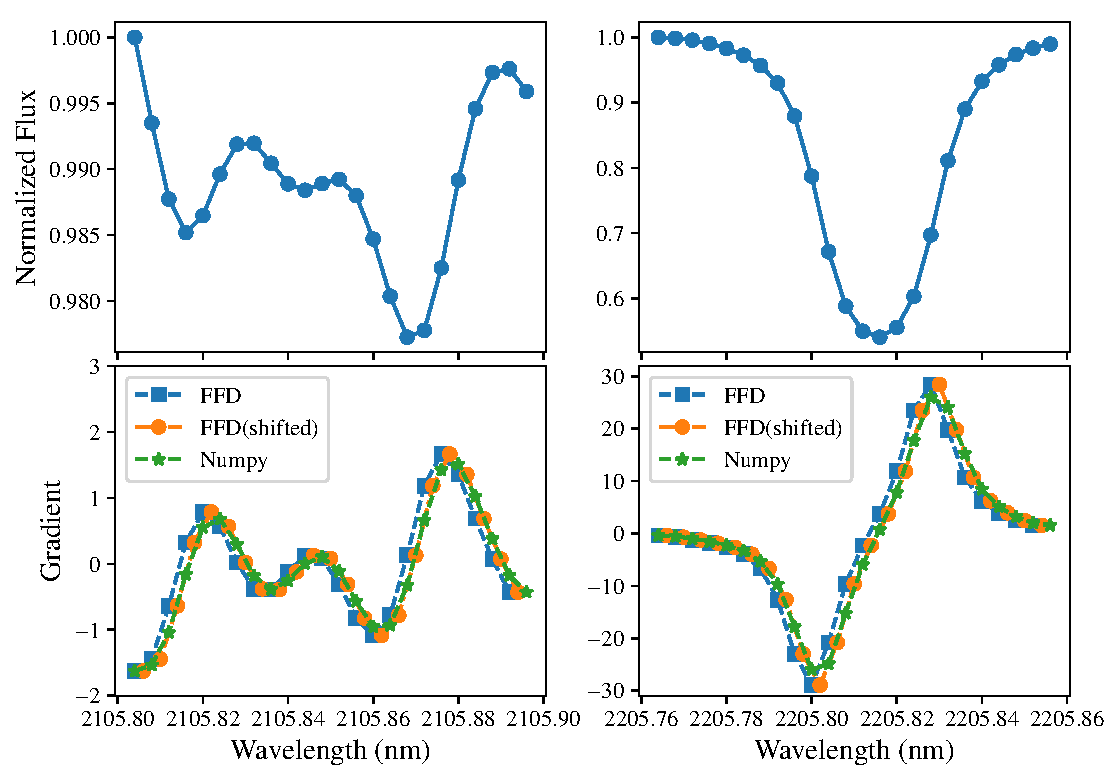
\includegraphics[width=0.8\linewidth]{figures/information-content/spectral_gradients}\\
    \caption[Comparing of numerical gradient alogithms.]{Visualization of the numerical gradient of some spectral lines.
        Top: The two spectral regions of a stellar spectrum the left hand slide contains short lines near the normalized continuum while on the right a single deep absorption line is shown.
        Bottom: The numerical gradients for the spectra shown in the top panels; the original {FFD} method is displayed with \emph{blue squares} while \numpy{} gradient is shown with \emph{green stars}.
        The \emph{orange circles} are the {FFD} version shifted to the mid-points between pixels for illustrative purposes.}
    \label{fig:gradients}
\end{figure}


%!TEX root = ../thesis.tex

\begin{table}
    \caption{The affect of the numerical gradient function on RV precision. The band label \(\rm VIS\) indicates the visible band while  \(\rm CARM_{VIS}\)  and \(\rm CARM_{NIR}\)  indicate the two wavelength bands of the CARMENES spectrograph. \(\Delta\lambda\) is a wavelength shift applied to analyse the pixel weights at the middle of their FFD gradients for comparison only.}
    \begin{tabular}{ccccccc}
        \toprule
%% Band & $\lambda$ range\_min & wl\_max &  dy/dx   & gradient & Q(dy/dx) & Q(grad) & Q(frac) & RV(dy/dx) & RV\_adj &    RV(grad)    &    RV(frac\_grad)    & RV(frac\_adj)          \\
  &   $\lambda$ range & \multicolumn{3}{c}{RV\(_{rms}\) (\mps{})} & \(\Delta\) RV ratio& \(\Delta\) RV ratio\\
 Gradient method&  &  A &   B & C & (B-A)/A & (C-A)/A \\
 Band  &  \si{\micro\meter} & FFD & FFD+\(\Delta\lambda\) &  CFD &  \% & \% \\
    \midrule
VIS & 0.38 -- 0.78 & 16.1 & 16.2 & 16.9  & 0.6 & 4.9\\
\(\rm CARM_{VIS}\) & 0.52 --  0.96 & 20.9 & 21.0 & 22.0 & 0.3& 5.2 \\
Z & 0.83 -- 0.93 & 76.9 & 77.0 & 78.8  & 0.1 & 2.5\\
Y & 1.00 -- 1.10 & 78.3 & 78.5 & 83.8 & 0.2 & 7.0 \\
J & 1.17 -- 1.33 & 149.3 & 149.4 & 156.4 & 0.1 & 4.7 \\
H & 1.50 -- 1.75 & 119.4 & 119.5 & 122.3 & 0.1 & 2.5 \\
K & 2.07 -- 2.35 & 153.4 & 153.7 & 157.7  & 0.2 & 2.8\\
\(\rm CARM_{NIR}\) & 0.96 -- 1.71 & 46.1 & 46.2 & 48.0 & 0.1& 4.2 \\
NIR & 0.83 -- 2.35 & 36.9 & 36.9 & 38.2 & 0.1 & 3.6  \\
    \bottomrule
    \end{tabular}\label{tab:numerical_gradients}
\end{table}


In \cref{fig:gradients} \todo{we} visualize the gradients of two small spectral regions computed with the original {FFD}, and the higher precision version incorporated in \numpy{}'s gradient function.
The top panels contain the spectrum in the small regions shown, indicating a large spectral line and three small lines near the continuum respectively.
The derivative of the spectra is shown in the bottom panel with the {FFD} method shown with \emph{blue squares} and the \numpy{} gradient shown in \emph{green stars}.
The \emph{orange circles} are the same as {FFD} but shifted horizontally to the midpoints between pixels.
This is for illustrative purposes and to assess the effect of this offset when calculating the pixel weights.

There a three notable features observed between gradient methods.
The first, which is expected from the {FFD} formulation is that the {FFD} gradient is offset to the left.
The second is that when the horizontal offset is adjusted (orange circles) the gradients lie along the same curve.
Both methods are trying to approximate the real gradient function of the spectrum and is again expected.
The most important feature observed in this though is that there is a slight over-estimate of the gradient by the {FFD} method at the peaks.
In the bottom panels of \cref{fig:gradients}, the points of highest gradient are always from the {FFD} method (blue/orange).
This is the case for all spectral lines and as the optimal pixel weights are proportional to the gradient squared the {FFD} method will apply slightly higher pixel weights to these values, two points per line in the spectrum.
The {FFD} will therefore produce a slightly smaller \(\delta V_{\rms}\) error compared to the more precise gradient function.

In \cref{tab:numerical_gradients} \todo{we} calculate the  \(\delta V_{\rms}\) using both gradient methods to determine their relative effect on the {RV} precision.

We took a {PHOENIX-ACES} spectrum with \Teff{}=3900\K{}, corresponding to {{M0}} spectral type.
The full theoretical precision is calculated (no telluric masking applied) with no rotational or instrumental broadening and the maximum of the continuum of each band scaled to 1.
In this case the {RV} precisions are not comparable between bands and are only to assess the direct effect of the changing the numerical gradient.
The bands name and the spanned wavelength are given.
The columns A, B, C are the {RV} precision for the different gradient methods.
The \(\delta V\) ratios are the relative difference in {RV} when changing from method A (the original {FFD}) to methods B and C.
In this table column B is the {FFD} method but with the wavelength shifted to in between pixels, corresponding to the orange circles in \cref{fig:gradients} while column C is the more precise gradient from \numpy{}.

We find that changing to use the gradient from \numpy{} increases the \(\delta V_{\rms}\) by 2.5--7\%, (decreasing the {RV} precision), due to the over-estimated gradient from the {FFD} method.
As the pixel weights \cref{eqn:optimal_weight} are also proportional to \({\lambda}^{2}\) column B was computed to assess the effect of the slight wavelength offset on the {RV} precision, visible in \cref{fig:gradients}.
This small wavelength shift red-ward does changed the {RV} precision by 0.1--0.6\% which is an order of magnitude smaller than the relative change when using \numpy{}'s gradient method.

Changing the method of numerical derivatives will change all the precision values given in the~\citet{figueira_radial_2016}.
This is a small impact on the precision compared to other components of the {RV} precision.
For instance from \cref{eqn:rv_SNR} a increase in \(\delta V_{\rms}\) of between 2.5--7\%  could equally be caused by a small decrease in the \snr{} from 100 (the value used in~\citet{figueira_radial_2016}) to between 95--98.

The current version of the software is now implemented with the gradient method provided by \numpy{} package.

\subsection{Masking Function}
\label{subsec:masking_function}
Another change made to the software is in the application of the masking function, and the treatment of telluric lines.
As suggested in~\citet{connes_absolute_1985} and~\citet{bouchy_fundamental_2001} a custom masking function can be applied to the individual pixel weights in \cref{eqn:optimal_weight}, such as:

\[W'(i) = W(i)M(i),\label{eqn:mask_function}\] where \(M(i)\) is the masking function and \(W'(i)\) are the modified pixel weights.
This masking function can be used in particular for the removal of telluric lines, setting those weights to zero and is in essence what is done when wavelength selection is performed; assigning zero weight to all pixels outside the desired wavelength range.

This masking function can be used to easily apply the three conditions presented in~\citet{figueira_radial_2016}.
First the 3 masking functions will be defined, then followed by the quantification of how they differ from the previous implementation.
The subscripts on the masking functions correspond to the three conditions.
\begin{align}
M_1(i) &= 1 \label{eqn:mask1}\\
M_2(i) &= \begin{cases}
0, \hspace{1em} T(i) < \tau\\
1, \hspace{1em} T(i) \ge \tau\\
\end{cases}\label{eqn:mask2}\\
M_3(i) &= {T(i)}^{2} \label{eqn:mask3}
\end{align}

Here, \(T(i)\) is the telluric transmission spectrum, while \(\tau\) is the transmission depth cut-off.
For instance to mask out telluric lines deeper than 2\%,  \(\tau\) would be set at 0.98.

\begin{itemize}
    \setlength\itemsep{-0.2em} % Remove spacing on list.
    \item Condition~\#1:
    The first mask, \(M_1\), is the simplest case in which all pixel weights are treated equally.
    No telluric line masking is considered.
    
    \item Condition~\#2:
    In the second mask, \(M_2\), the telluric line transmission, \(T(i)\) is used to create a boolean mask of 0's and 1's.
    When applying this mask to the pixel weights, the pixels effected by telluric lines have 0 weight, removing their contribution to the {\red{} \(RV_{\rms}\)}.
    Accounting for seasonal variation in Earth's barycentric motion can be easily incorporated into this mask, widening the regions masked out.
    
    \item Condition~\#3:
    The third mask, \(M_3\), assumes the application of perfect telluric correction consistent with Condition~\#3.
    The pixel weights are modified by dividing the flux variance by the square of the transmission spectrum\reference{cite the equation when I refer to it}.
    As the flux variance is the denominator of \cref{eqn:optimal_weight}, this is equivalent to multiplication of the weights by a mask of the form \(M_3\).
\end{itemize}

Having the three masks defined in this way makes the implementation of the {RV} precision simpler.
In the original version there were three separate implementations, one for each condition.
With this, \todo{Check this if it is previous}{as mentioned previously} there was a issue with the implementation of Condition~\#2.

\subsubsection{Masking order}
\label{subsubsec:masking_order}
The order in which the masking is performed is also important.
Masking should be applied only after calculation of the pixel weights.
As the pixel weights depend on neighbouring points (through the calculation of the gradients), prematurely removing pixels will affect the precision results.

The original implementation of Condition~\#2 did just this, splitting the spectra into small sections in between the masked off telluric lines.
The {\red{}\(RV_{\rms}\)} is calculated for each section and then the results are combined as the error on the weighted average in \cref{eqn:weighted_average_error}.
Analytically this identical to masking the pixel weights with \(M_2\) but not in practice when numerically implemented.
\todo{Should I show the working of analytical working out of this in an appendix, or here?}

When the spectrum is split into small sections the number of edges increases and the number of pixels affected by any edge effects increases.
Using the {FFD} method to compute the gradient the last pixel is removed/lost.
A spectrum split in \(m\) sub-spectra will therefore lose \(m\) pixels due to edge effects (instead of only 1 pixel with the full spectrum).
Even the \numpy{} gradient is not immune to the edge effects in the sub-spectra when splitting the spectrum first.
Even though there is no pixels lost, the first and last pixels of each sub-spectra are computed using forward or backward differences, rather than central differences (as they would be in the full spectrum).
Hence the gradients and weights of some pixels are slightly changed due to the splitting occurring first.

We quantify the effect of splitting the spectrum before and after calculating the weights in \cref{tab:mask_ordering}.
The columns label \emph{Split} represents splitting the spectrum before calculating the pixel weights while the \emph{Mask} columns calculate all the pixel weights first and then apply the \(M_2\) mask.
The difference in {RV} precision between both situations and for both gradient methods are given.
For the {FFD} gradient the ordering of masking changes decreases the {\red{}\(RV_{\rms}\)} by 0.2--0.7\%, while for the \numpy{} gradient it is increase but an order of magnitude smaller between 0.01--0.13\%.
The {FFD} gradient is causes a larger difference as points that were masked out are now included where as with the \numpy{} gradient the end values are always included but their gradients are slightly changed.
The last column is the difference ratio between the \emph{Mask} column of both gradient method, this is consistent with \cref{tab:numerical_gradients} with the differences from two gradient methods between 2--7\%.
It shows that the difference from changing order of masking is 1--2 orders of magnitude smaller than changing the gradient method.

The code has been adjusted to consistently apply the masking after the pixel weights are calculated.
This retains the most pixels, with the more accurate pixel weights.
It has also been changed to just apply \(M_2\) rather than splitting and performing the weighted error calculation.
\todo{did I check this was equivalent} This simplifies the implementation in calculating the {RV} precision.

%!TEX root = ../thesis.tex

\begin{table}
    \centering
    \caption{Relative {RV} precision difference for Condition \#2 due to spectral splitting and order of applying the pixel mask. The ratio are the difference between Split and Masked implementations with the same gradient calculation. The last column is the ratio between the Masked versions using the FFD and numpy gradient methods and are consistent with \tref{tab:numerical_gradients}. Results a for an M0 spectral type, with vsini=1.0 and R=100,000.}
    \begin{tabular}{c|ccc|ccc|c}
        \toprule
        & Split & Masked & \(\Delta\)Ratio & Split & Masked & \(\Delta\)Ratio & Masked \\
        Gradient & \multicolumn{3}{c|}{FFD} & \multicolumn{3}{c|}{Numpy} & \(\Delta\)Ratio\\
        Band & \mps{} & \mps{} &  \%  & \mps{} & \mps{} &   \% & \% \\
        \midrule
        Z &  7.42 &  7.38 & -0.66 &  7.76 &  7.77 & 0.13 & 5.3\\
        Y &  4.75 &  4.74 & -0.22 &  5.06 &  5.06 & 0.06 & 6.8\\
        J & 18.58 & 18.53 & -0.29 & 19.57 & 19.57 & 0.01 & 5.6\\
        H &  6.08 &  6.05 & -0.53 &  6.25 &  6.26 & 0.08 & 3.5\\
        K & 32.21 & 32.14 & -0.22 & 33.48 & 33.49 & 0.05 & 4.2\\
        \bottomrule
    \end{tabular}\label{tab:mask_ordering}
\end{table}

{\rd{} The results from these spectra for conditions \#1 and \#3 are consistent with Figueira et al. 2016. \todo{put this some where}}


{\red{} For Condition~\#2 in which there was an error there is no meaningful relation between the new and old values.
    \todo{put this line elsewhere.}}


\subsection{\snr{} scaling}
\label{subsec:snr_scaling}
To analyse the relative precision of different spectra they need to normalized to a common reference point.
In this section \todo{we} detail how this was originally done and how this was changed to be adaptable to any library spectra and any reference band.

In the original code this was selected to be a \snr{} per pixel of 100 at the centre of the \textit{J}-band at 1.25\si{\micro\meter}.
The normalization values for each band, \Vsini{} and resolution combination were hard-coded into the analysis.
This made it impossible to easily adapt the code to other spectra or parameter combinations.

An automated \snr{} scaling procedure was created to remove the hard-coded values.
This updated code finds the centre point of the band of reference for the given spectrum.
Totals the photon count across one resolution element, \(\delta\lambda\), and then takes the square root.
This is using the definition of the \snr{} as \(\snr{} = \sqrt{N}\) for large N.
This value is then used to scale the spectrum such that the \snr{} at the reference point is the desired value.
\begin{equation}
SF =  \frac{\sqrt{\sum{\delta\lambda} A}} {\snr{}_{desired}}
\end{equation}
\textit{SF} where \textit{SF} is the scaling factor, \(\sum_{\delta\lambda} A\) is the sum of the point in one resolution element and \({\snr{}}_{desired}\) is the desired \snr{} level requested.

This automated procedure enabled {\red{}\textbf{4}} different features.
\begin{itemize}
    \setlength\itemsep{-0.3em} % Remove spacing on list.
    \item The ability to analysis other spectral models, not just corresponding to {M0}, {M3}, {M6}, {M9} spectral types.
    - Scaling to a \snr{} per pixel level other than 100.
    \item A \snr{} per pixel other than 100 can be selected.
    - Allowing for other sampling levels (if desired)
    \item Not restricted to a model with 3 samples per resolution element.
    \item Different reference bands available.
    Results are not limited to being referenced from the \textit{J}-band.
    For instance the {RV} precision can now be calculated for a given \snr{} at the centre of the \textit{K}-band.
    This was one the features requested for the Exposure Time Calculators precision values.
    For {NIRPS} \todo{we} provided precision values relative to each individual band, while for {SPIRou} they were relative to the {J}- and {H}-bands.
\end{itemize}

The default values for the \snr{} scaling a still 100 at the centre of the \textit{J}-band, but there is now options to easily change these values.

The centre of each band was visually checked to ensure that there were no spectral lines at the reference locations> If a line was present at the reference point its depth variability across spectral types would affect the \snr{} scaling levels at a greater than the normal change in continuum amplitude/shape.\todo{is this needed}

As shown in \cref{eqn:snr_relation} the {RV} precision is inversely proportional to the \snr{} level.
To access the {RV} precision of any of the values in Table at a different \snr{} level you can apply the following
\begin{equation}
{RV}_{{\snr{}}_{2}} = {RV}_{{\snr{}}_{1}} * \frac{{\snr{}}_{1}}{{\snr{}}_{2}}.
\end{equation}

\todo{\snr{} plot/diagram}



\subsection{Atmospheric masking bug}
\label{subsec:condition_two_bug}
Applying testing practises revealed a error in the application of Condition~\#2 in \citep{figueira_radial_2016}.
When the telluric line mask was broadened to account for the barycentric motion of the Earth, and the requirement requiring three consecutive pixels (the sampling rate) to exceed the cut-off limit to be considered masked out there was a software bug.

This meant that the masking applied for Condition \#2 was garbage, and not physically meaningful.
Essentially randomly masking portions of the spectra.
The synthetic spectra did not have telluric contamination present but the proportion and location of the telluric masking applied was incorrect.

A check for this issue was discovered using this unit test, written under the \href{https://docs.pytest.org}{pytest} framework.
Essentially, this takes a given transmission (telluric line) spectrum and creates a telluric mask at a line depth of 2\%.
It then transforms the mask by the function \emph{barycentre\_broaden()}, the function under test here, which performs the \(\pm30\)\kmps{} barycentre broadening to account for the yearly motion of the Earth, and consecutive pixel check.
The assert statement performs the actual test, checking that if the new broadened mask is applied to the original transmission spectrum, then all values are greater or equal to the masking limit.
That is the telluric lines are still completely masked out.

This is not the only test required to sufficiently test the ``correctness'' of \emph{barycentre\_broaden()}, but it is a simple unit test\footnote{A unit test only tests  single specific piece of code or functionality at a time.} that would have caught the bug that was present.
\begin{lstlisting}[language=Python, caption=Example unit test to catch the masking bug.\ The assert statement checks that the mask continues to remove all telluric lines deeper than 2\%.]
def test_telluric_masking(wavelength, transmission):
    """Check the mask still masks out all telluric lines > 0.98 
    after broadening the mask to
    accounting for the barycentre motion."""
    mask = telluric_mask(transmission, depth=0.98)  # Create mask
    mask = barycentre_broaden(wavelength, mask)     # Extend mask
    assert numpy.all(transmission[mask] >= 0.98)    # Assert something about mask
\end{lstlisting}

Due to this bug the published {RV} precision values for Condition~\#2  in~\citet{figueira_radial_2016} are all incorrect.
As the masking was unevenly applied the new ``correct'' {RV} precision values do not all change in the same direction or in the same proportion.
For example largest difference is seen in the \emph{J}- and \emph{K}-bands, with changes over 20\mps{}, whil other wavelength bands are essentially unchanged.
The differences can be seen in the shaded areas of \cref{fig:figueria_comparision} comparing the \citet{figueira_radial_2016} results to the updated values, with the upper edge defined by Condition \#2.
Even though there is an error with the values of condition~\#2 they do not change the overall conclusions of the paper.
